\chapter{Parallelisation of the Problem}
Given the typically $O(n^2)$ behaviour of the longest common sub-sequence problem, one way of accelerating the computation time is to break the problem up into distinct subsections and approach it in parallel. The following sections describe the approach taken to paralleise the problem using the OpenMP and Open MPI C++ libraries.

\section{Parallelisation Strategy}

% How did I make use of OpenMP?
\subsection{Multi-Threading with OpenMP}
Due to the fact that multiple threads can be run in a single process and that OpenMP utilises threads for its multi-processing, I decided early on that in order to maximise the performance of the program that the OpenMP optimisations would take place inside each MPI process.

Utilising OpenMP effectively proved challenging and required a complete overhaul of the serial code for populating the table described in Section 1.2 and visualised in Figure \ref{fig:table}. Instead of populating the table iteratively by row and column, cells were populated on the anti-diagonal (see Figure \ref{fig:techniques}). Because each cell only relies on the cells to its left and top, this allows every cell the entire anti-diagonal to be calculated simultaneously. In theory, if the same number of OpenMP threads were allocated to length of the diagonal, each cell in that diagonal could be calculated independently (and in parallel.

\begin{figure}[h]
\label{fig:techniques}
\centering
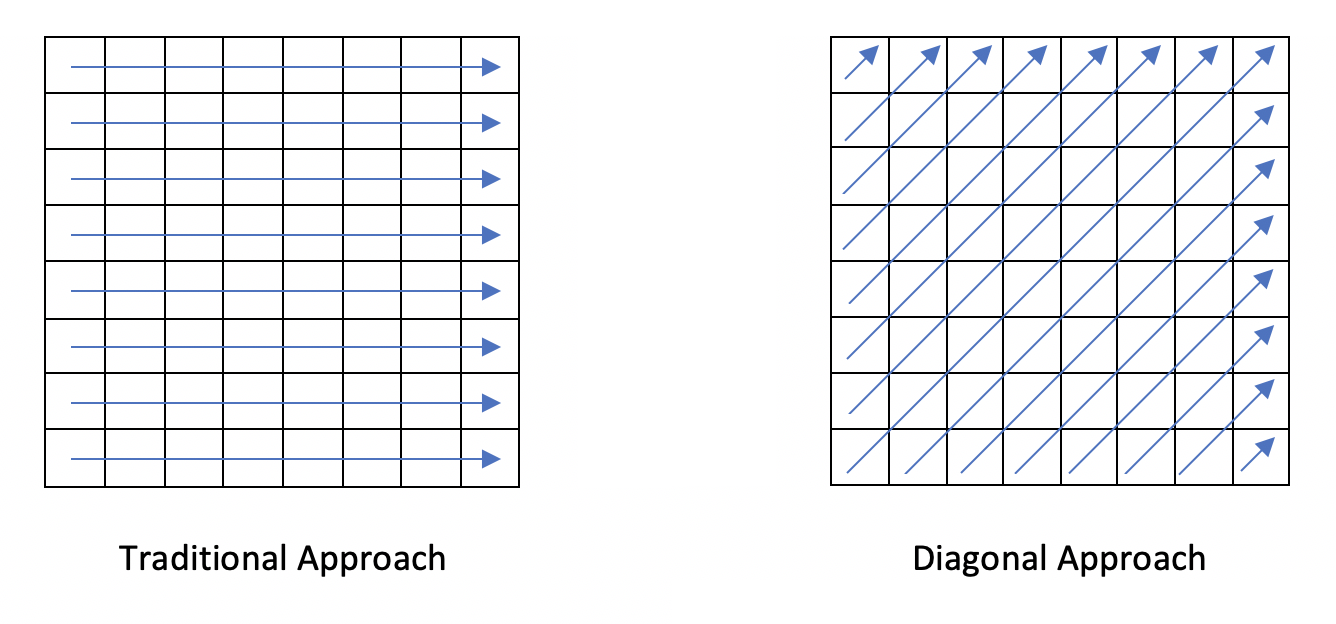
\includegraphics[width=12cm]{img/diagonal.png}
\caption{Population Techniques}
\end{figure}

This required the pre-computation of an order of execution more complicated than iterating over the length and height of the matrix. A C++ \lstinline{vector<vector<int>>} object was used to store the co-ordinates of each cell making up each "diagonal." These diagonals were then processed iteratively, with each constituent cell being processed in parallel using an OpenMPI \lstinline{parallel for} construct (see Listing 2.1).

\begin{lstlisting}[language=C++, caption=OpenMP Utilisation]
// The variable indices is vector<vector<int>> containing a list of diagonals
// which themselves contain (x, y) co-ordindate pairs.
for (int i = 0; i < (int) indices.size(); i++) {
    vector<vector<int>> diagonal = indices[i];
    #pragma omp parallel for shared(table, diagonal, a, b, top, left)
    for (int j = 0; j < (int) diagonal.size(); j++) {
        vector<int> cell = diagonal[j];
        int x = cell[0];
        int y = cell[1];
        int result = calculate_cell(table, x, y, a, b, top, left);
        table[y][x] = result;
    }
}
\end{lstlisting}

% How did I make use of MPI?
\subsection{Multi-Processing with OpenMPI}
Transforming the program so that it could make use of multiple processes was incredibly challenging. Splitting up the problem space into neat sub-sections was non-trivial, when accounting for the potential of irregularities around the "edges" of the parent matrix (i.e. "non-full" sections). The order in which the segments are processed is practically identical to that of the OpenMP calculations for each cell, but instead of individual cells being computed in parallel by threads, whole sections are computed in parallel by MPI processes (each internally using OpenMP for cell-level calculations). 

The number of processes provided to the program is fetched dynamically and determines the number of segments. One process is reserved for the parent or "master," with remainder being used as child, or "worker" processes. The number of segments in the anti-diagonal is matched to the number of processes so that at peak parallelism (when the most cells are able to be processed in parallel), the program can take full advantage.

In figure \ref{fig:segmentation} below, the program has been allocated five processes, four of which have been made worker processes. This has resulted in a diagonal size of four, and a total sub-section count of sixteen. Each set of sub-sections of the same colour represent "diagonals." Each sub-section in a diagonal can have its constituent cell values calculated in parallel with those of the other sub-sections in that diagonal. The white arrow indicates the direction that diagonals are processed. The red and violet sections (the first and last diagonals) are processed by the master process due to either being necessary for the first worker processes or requiring the output of all previous cells, respectively.

\begin{figure}[h]
\centering
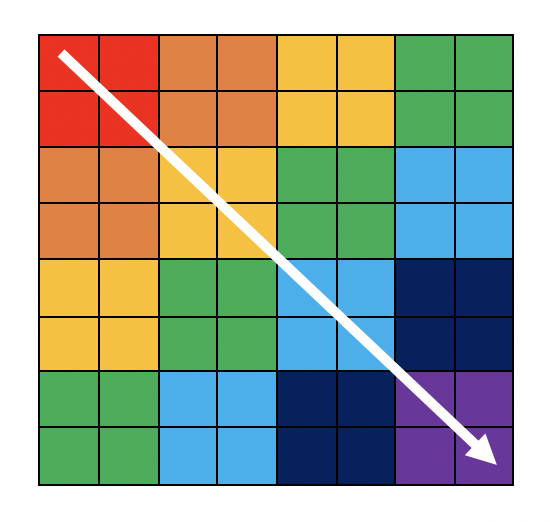
\includegraphics[width=5cm]{img/segments.png}
\caption{MPI Segmentation Technique}
\label{fig:segmentation}
\end{figure}

% How is information shared between threads and processes?
\subsection{Information Sharing}
\subsubsection{OpenMP}
Passing information to OpenMP was trivial due to the fact that each thread wrote to a discrete set of cells and read from cells that had already been populated (and would remain unchanged) in the calculation of the previous diagonal. In light of this, the master table was simply passed to each thread

\subsubsection{MPI}
Passing information was significantly more difficult between processes and required the use of the MPI message passing interface. For the computation of each sub-section additional data is required from the adjoining cells to the top and left. Figure \ref{fig:topleft} shows a single sub-segment (in orange) and the "top" (in blue) and "left" (in red) required to compute it. Each child, on inception, blocks and waits (using \lstinline{MPI_Recv()}) for three batches of information: the co-ordinates of the corners of the section being computed, the "top" data (converted into a one-dimentional \lstinline{int} array), and the "left" data (also converted), which are sent (using \lstinline{MPI_Send()}) by the master process. After computation, the contents of the subsection (in one-dimenional format) are sent back to the master process and are used to populate the master table.

\begin{figure}[h]
\centering
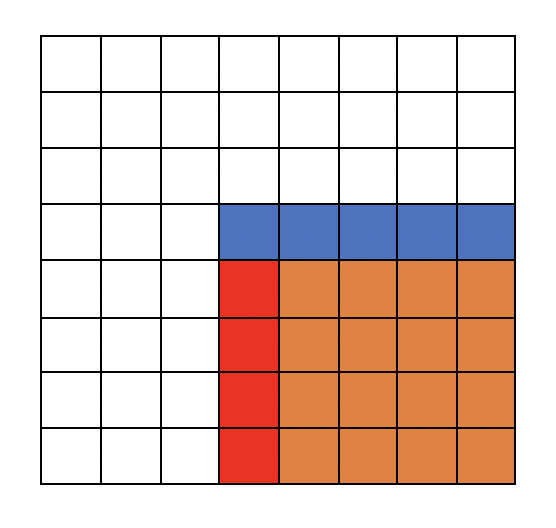
\includegraphics[width=5cm]{img/topleft.png}
\caption{Top (Blue) and Left (Red) Sections}
\label{fig:topleft}
\end{figure}

% Any optimisations investigated and/or challenges encountered will go here
\subsection{Challenges}
There were numerous false starts when devising a hybrid solution to the LCS problem. One particular example was a method devised by \cite{Li2017}. However, upon implementation it became apparent that the algorithm provided had several errors. It proved easier implementing, from scratch, the logic for handling both the OpenMP and MPI portions of the program.

Resource access was also a point of difficulty, particularly when trying to run tests with more than one or two processes (let alone multiple nodes) in the week leading up to the submission of milestone two.

Edge cases surrounding the behaviour of the program when assigned less than three processes were also encountered, overcome by reverting the application to utilising only OpenMP in these cases.

It also proved infeasible to parallelise the reconstruction of the longest common subsequence from the table (backtracking), as each step relied on the state acheived by the previous one. Many possibilities were considered but the nature of the problem procluded any obvious speedups from either OpenMP or MPI.

% A description of how you have verified the correctness of your parallel implementation. 
\section{Verification}
Due to the increased complexity of the code when deconstructing the problem to be performed over multiple threads and multiple processes it was essential to verify that the correctness of the program was maintained. The test suite from Section \ref{sec:correctness} was rerun under each of the following conditions:

\begin{itemize} 
    \item With a single MPI process.
    \item With three MPI processes (the lowest size that will trigger MPI multi-processing).
    \item With four MPI processes (typical usage).
    \item With sixteen MPI processes (high usage).
\end{itemize}

Each of these tests was run with an allocation of a single OpenMP thread (effectively serial), then again with with multiple threads.

\section{Scalability Test Plan}

\subsection{Strong Scaling}
Strong scaling measures the increase in performance for a fixed problem size. To test this form of scaling, two randomly generated strings of 100,000 each will be generated and run with the configurations in Table \ref{tab:strong}. These vary over two primary parameters: number of processes and number of threads. Due to the nature of the test clusters, when the number of processes exceeds the available number of CPU cores on a node, multiple nodes are used and the processes are split up evenly over multiple nodes.

\begin{table}[H]
\centering
\begin{tabular}{|l|l|l|l|}
\hline
\textbf{Nodes} & \textbf{\begin{tabular}[c]{@{}l@{}}Number of Tasks\\ (processes)\end{tabular}} & \textbf{Number of Tasks Per Node} & \textbf{\begin{tabular}[c]{@{}l@{}}CPUs Per Tasks\\ (threads)\end{tabular}} \\ \hline
1 & 1 & 1 & 1 \\ \hline
1 & 2 & 2 & 2 \\ \hline
1 & 4 & 4 & 4 \\ \hline
1 & 8 & 8 & 8 \\ \hline
1 & 16 & 16 & 8 \\ \hline
1 & 16 & 16 & 16 \\ \hline
1 & 16 & 16 & 32 \\ \hline
2 & 32 & 16 & 8 \\ \hline
2 & 32 & 16 & 16 \\ \hline
2 & 32 & 16 & 32 \\ \hline
4 & 64 & 16 & 32 \\ \hline
\end{tabular}
\caption{Strong Scaling Plan}
\label{tab:strong}
\end{table}

These runs will be run on UQ's \lstinline{goliath} cluster using \lstinline{slurm} (\lstinline{sbatch}) and a configuration shell script. An example script has been included in Appendix 3. Each run will be timed and compared to the serial solution and one another. The comparison with the serial solution will allow for the determination of how effective the solution is with respect to strong scaling or "speed up."

\subsection{Weak Scaling}
Weak scaling measures the effect of a program's parallelism as the size of the input changes. To test this type of scaling, I will run the same tests used for each of the following randomly generated string lengths:

\begin{table}[H]
\centering
\begin{tabular}{|l|}
\hline
\textbf{Input Length} \\ \hline
1 \\ \hline
10 \\ \hline
100 \\ \hline
1000 \\ \hline
10000 \\ \hline
100000 \\ \hline
\end{tabular}
\caption{Weak Scaling}
\label{tab:weak}
\end{table}

In order to offset any abnormalities caused by particular (randomly generated) input strings, each test will be run multiple times and averaged out. The \lstinline{testing.py} script used for the first milestone will be modified to support this behaviour.

% The idea here is that you could take this plan an start performing timing experiments. You should arrange testing so that if your test plan is curtailed, then you can still draw sensible conclusions from the results you do get.

\subsection{Test Plan Timeline}
In order to avoid the trouble I faced with respect to node availability, I expect to front-load a lot of the work for the final milestone. The table below outlines my timeline:

\begin{table}[H]
\centering
\begin{tabular}{|l|l|l|}
\hline
\textbf{Week} & \textbf{Activity} & \textbf{Rationale} \\ \hline
Midsemester Break & \begin{tabular}[c]{@{}l@{}}Development of testing.py \\ script for automating testing\end{tabular} & \begin{tabular}[c]{@{}l@{}}Automating the testing will save the \\ manual entry of parameters\end{tabular} \\ \hline
Week 11 & Strong Scaling & \begin{tabular}[c]{@{}l@{}}Strong scaling is the simple case and \\ can be tackled first\end{tabular} \\ \hline
Week 12 & Weak Scaling & \begin{tabular}[c]{@{}l@{}}This should be just the addition of extra \\ parameters (and iteration) to the strong scaling\end{tabular} \\ \hline
Week 13 & Buffer Time & \begin{tabular}[c]{@{}l@{}}I have left this space free in case testing\\  takes longer than expected, but would prefer\\  to avoid it as the clusters will be busy\end{tabular} \\ \hline
\end{tabular}
\caption{Timeline}
\label{tab:timeline}
\end{table}


% Remember that getafix is a shared facility so you are not guaranteed to get all the time you might like.
\clearpage